%%%%%%%%%%%%%%%%%%%%%%%%%%%%%%%%%%%%%%%%%
% Short Sectioned Assignment
% LaTeX Template
% Version 1.0 (5/5/12)
%
% This template has been downloaded from:
% http://www.LaTeXTemplates.com
%
% Original author:
% Frits Wenneker (http://www.howtotex.com)
%
% License:
% CC BY-NC-SA 3.0 (http://creativecommons.org/licenses/by-nc-sa/3.0/)
%
%%%%%%%%%%%%%%%%%%%%%%%%%%%%%%%%%%%%%%%%%

%----------------------------------------------------------------------------------------
%	PACKAGES AND OTHER DOCUMENT CONFIGURATIONS
%----------------------------------------------------------------------------------------

\documentclass[paper=a4, fontsize=11pt]{scrartcl} % A4 paper and 11pt font size

\usepackage[T1]{fontenc} % Use 8-bit encoding that has 256 glyphs
\usepackage{fourier} % Use the Adobe Utopia font for the document - comment this line to return to the LaTeX default
\usepackage[english]{babel} % English language/hyphenation
\usepackage{amsmath,amsfonts,amsthm} % Math packages

\usepackage{lipsum} % Used for inserting dummy 'Lorem ipsum' text into the template
\usepackage{graphicx}

\usepackage{sectsty} % Allows customizing section commands
%\allsectionsfont{\centering \normalfont\scshape} % Make all sections centered, the default font and small caps

\usepackage{fancyhdr} % Custom headers and footers
\pagestyle{fancyplain} % Makes all pages in the document conform to the custom headers and footers
\fancyhead{} % No page header - if you want one, create it in the same way as the footers below
\fancyfoot[L]{} % Empty left footer
\fancyfoot[C]{} % Empty center footer
\fancyfoot[R]{\thepage} % Page numbering for right footer
\renewcommand{\headrulewidth}{0pt} % Remove header underlines
\renewcommand{\footrulewidth}{0pt} % Remove footer underlines
\setlength{\headheight}{13.6pt} % Customize the height of the header

\numberwithin{equation}{section} % Number equations within sections (i.e. 1.1, 1.2, 2.1, 2.2 instead of 1, 2, 3, 4)
\numberwithin{figure}{section} % Number figures within sections (i.e. 1.1, 1.2, 2.1, 2.2 instead of 1, 2, 3, 4)
\numberwithin{table}{section} % Number tables within sections (i.e. 1.1, 1.2, 2.1, 2.2 instead of 1, 2, 3, 4)

\setlength\parindent{0pt} % Removes all indentation from paragraphs - comment this line for an assignment with lots of text

%----------------------------------------------------------------------------------------
%	TITLE SECTION
%----------------------------------------------------------------------------------------

\newcommand{\horrule}[1]{\rule{\linewidth}{#1}} % Create horizontal rule command with 1 argument of height

\title{	
\normalfont \normalsize 
\textsc{University of Freiburg} \\ [25pt] % Your university, school and/or department name(s)
\horrule{0.5pt} \\[0.4cm] % Thin top horizontal rule
\huge Exercise 2: Convolutional Neural Networks \\ % The assignment title
\horrule{2pt} \\[0.5cm] % Thick bottom horizontal rule
}

\author{Hendrik Vloet} % Your name

\date{\normalsize\today} % Today's date or a custom date

\begin{document}

\maketitle % Print the title

%----------------------------------------------------------------------------------------
%	PROBLEM 1
%----------------------------------------------------------------------------------------

\section{Theory}
\subsection{Convolutional Neural Networks}

This section is meant to provide a quick recap of Convolutional Neural Networks (CNNs), so I tried to keep it short.\\
A convolutional neural network is a feed-forward neural network that does not rely solely on fully connected layers. Typically a CNN consists of several layers that are designed in a way to detect more and more advanced features of the input data, the deeper the network propagates forth. This principle setup is shown in figure \ref{pic:example_cnn}
\begin{figure}[hbpt!]
	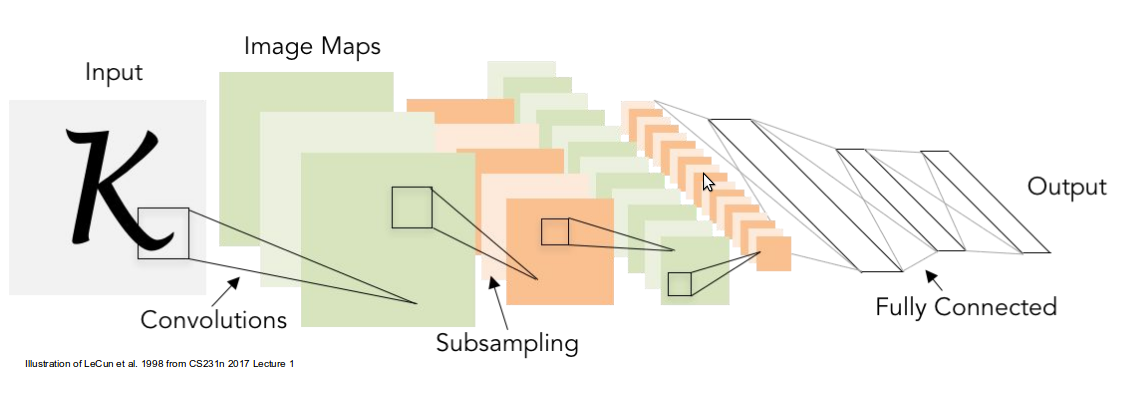
\includegraphics[width=\textwidth]{example_cnn}
	\label{pic:example_cnn}
	\caption{Example CNN, taken from LeCun et al. 1998 from CS231n 2017 Lecture 1}
\end{figure}
\clearpage

The basic workflow works like this:
\begin{enumerate}
	\setlength\itemsep{0em}
	\item Image is fed into the Network
	\item The image is convolved with several layers of various dimensions, e.g. 16 filters with dimensions 3x3
	\item depending on the convolution operation (same/valid), the image dimensions are changed, let's assume we use same convolution, i.e. the dimensions of the input image are not changed when going through a convolution layer.
	\item after convolution, there can be some sort of sub sampling in order to make the data more manageable. One example could be a 2x2 max pooling layer, which reduces the dimensions of its input data by half. So for example, if we fed an 28x28 image into a max-pool-2x2 layer, we get as output a lower resolved 14x14 image.
	\item By using more and more convolution and pooling layers, the network extracts more and more complex features from the original data, e.g. first it detects some contours, than edges and in the end it can classify an object with the help of these "high-level" features.
	\item The last stage is one fully connected layer, like in classic neural networks. It uses an activation and a loss function in order to get correct classification results. Note that the input of the fully connected layer is now longer an multi-dimensional image, but a flattened array according to the designed network.
	\item Finally the output of this network is a classification. 
\end{enumerate}

\subsubsection{Hyperparameters}
There are several hyperparameters for CNNs one can tweak, here is a short overview over the most common (there are many more):
\begin{itemize}
	\item Number of Layers
	\item Choice of Pooling
	\item Choice of Loss Function
	\item Filter dimensions
	\item Zero Padding
	\item same/valid convolution
	\item Stride
	\item convolution method:
	\begin{itemize}
		\item Convolution: $S(i,j) = (K \ast I)(i,j) = \sum \limits _m \sum \limits _n I(i-m,j-n)K(m,n)$
		\item Cross-Correlation: $S(i,j) = (I \ast K)(i,j) = \sum \limits _m \sum \limits _n I(i+m,j+n)K(m,n)$\\(flipping the kernel first and then applying cross-correlation is equivalent to convolution)
	\end{itemize}
\end{itemize}

%------------------------------------------------

\section{Task 1: Setup}

The general Setup as it is implmented is shown in figure CITE. It shows the most basic configuration, i.e. the parameters of Task 1. Dimensions are chosen accordingly and are of course modified later on for different filter depths.\\
I used a SGD optimising approach with a fixed batch size of 50.\\
I chose 20 epochs to train and test.
\begin{figure}[hbpt!]
	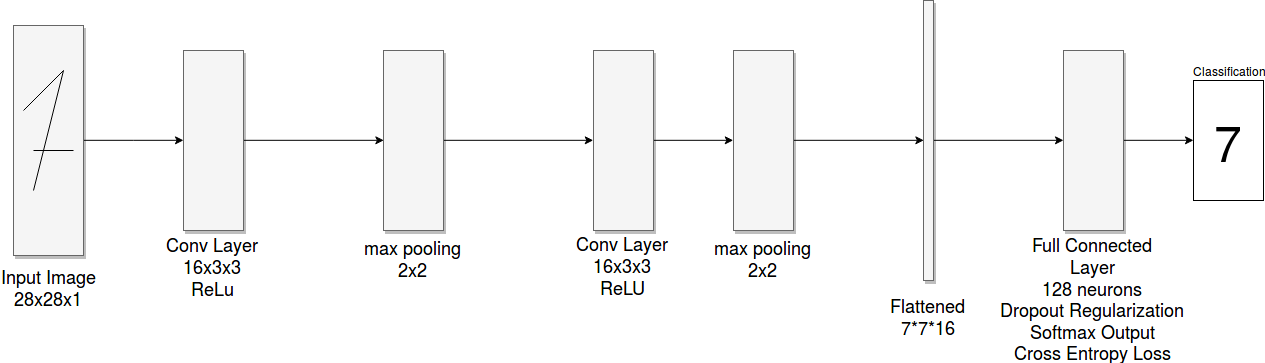
\includegraphics[width=\textwidth]{setup}
	\label{fig:setup}
	\caption{Principal structure of the used CNN}
\end{figure}
\begin{figure}[hbpt!]
	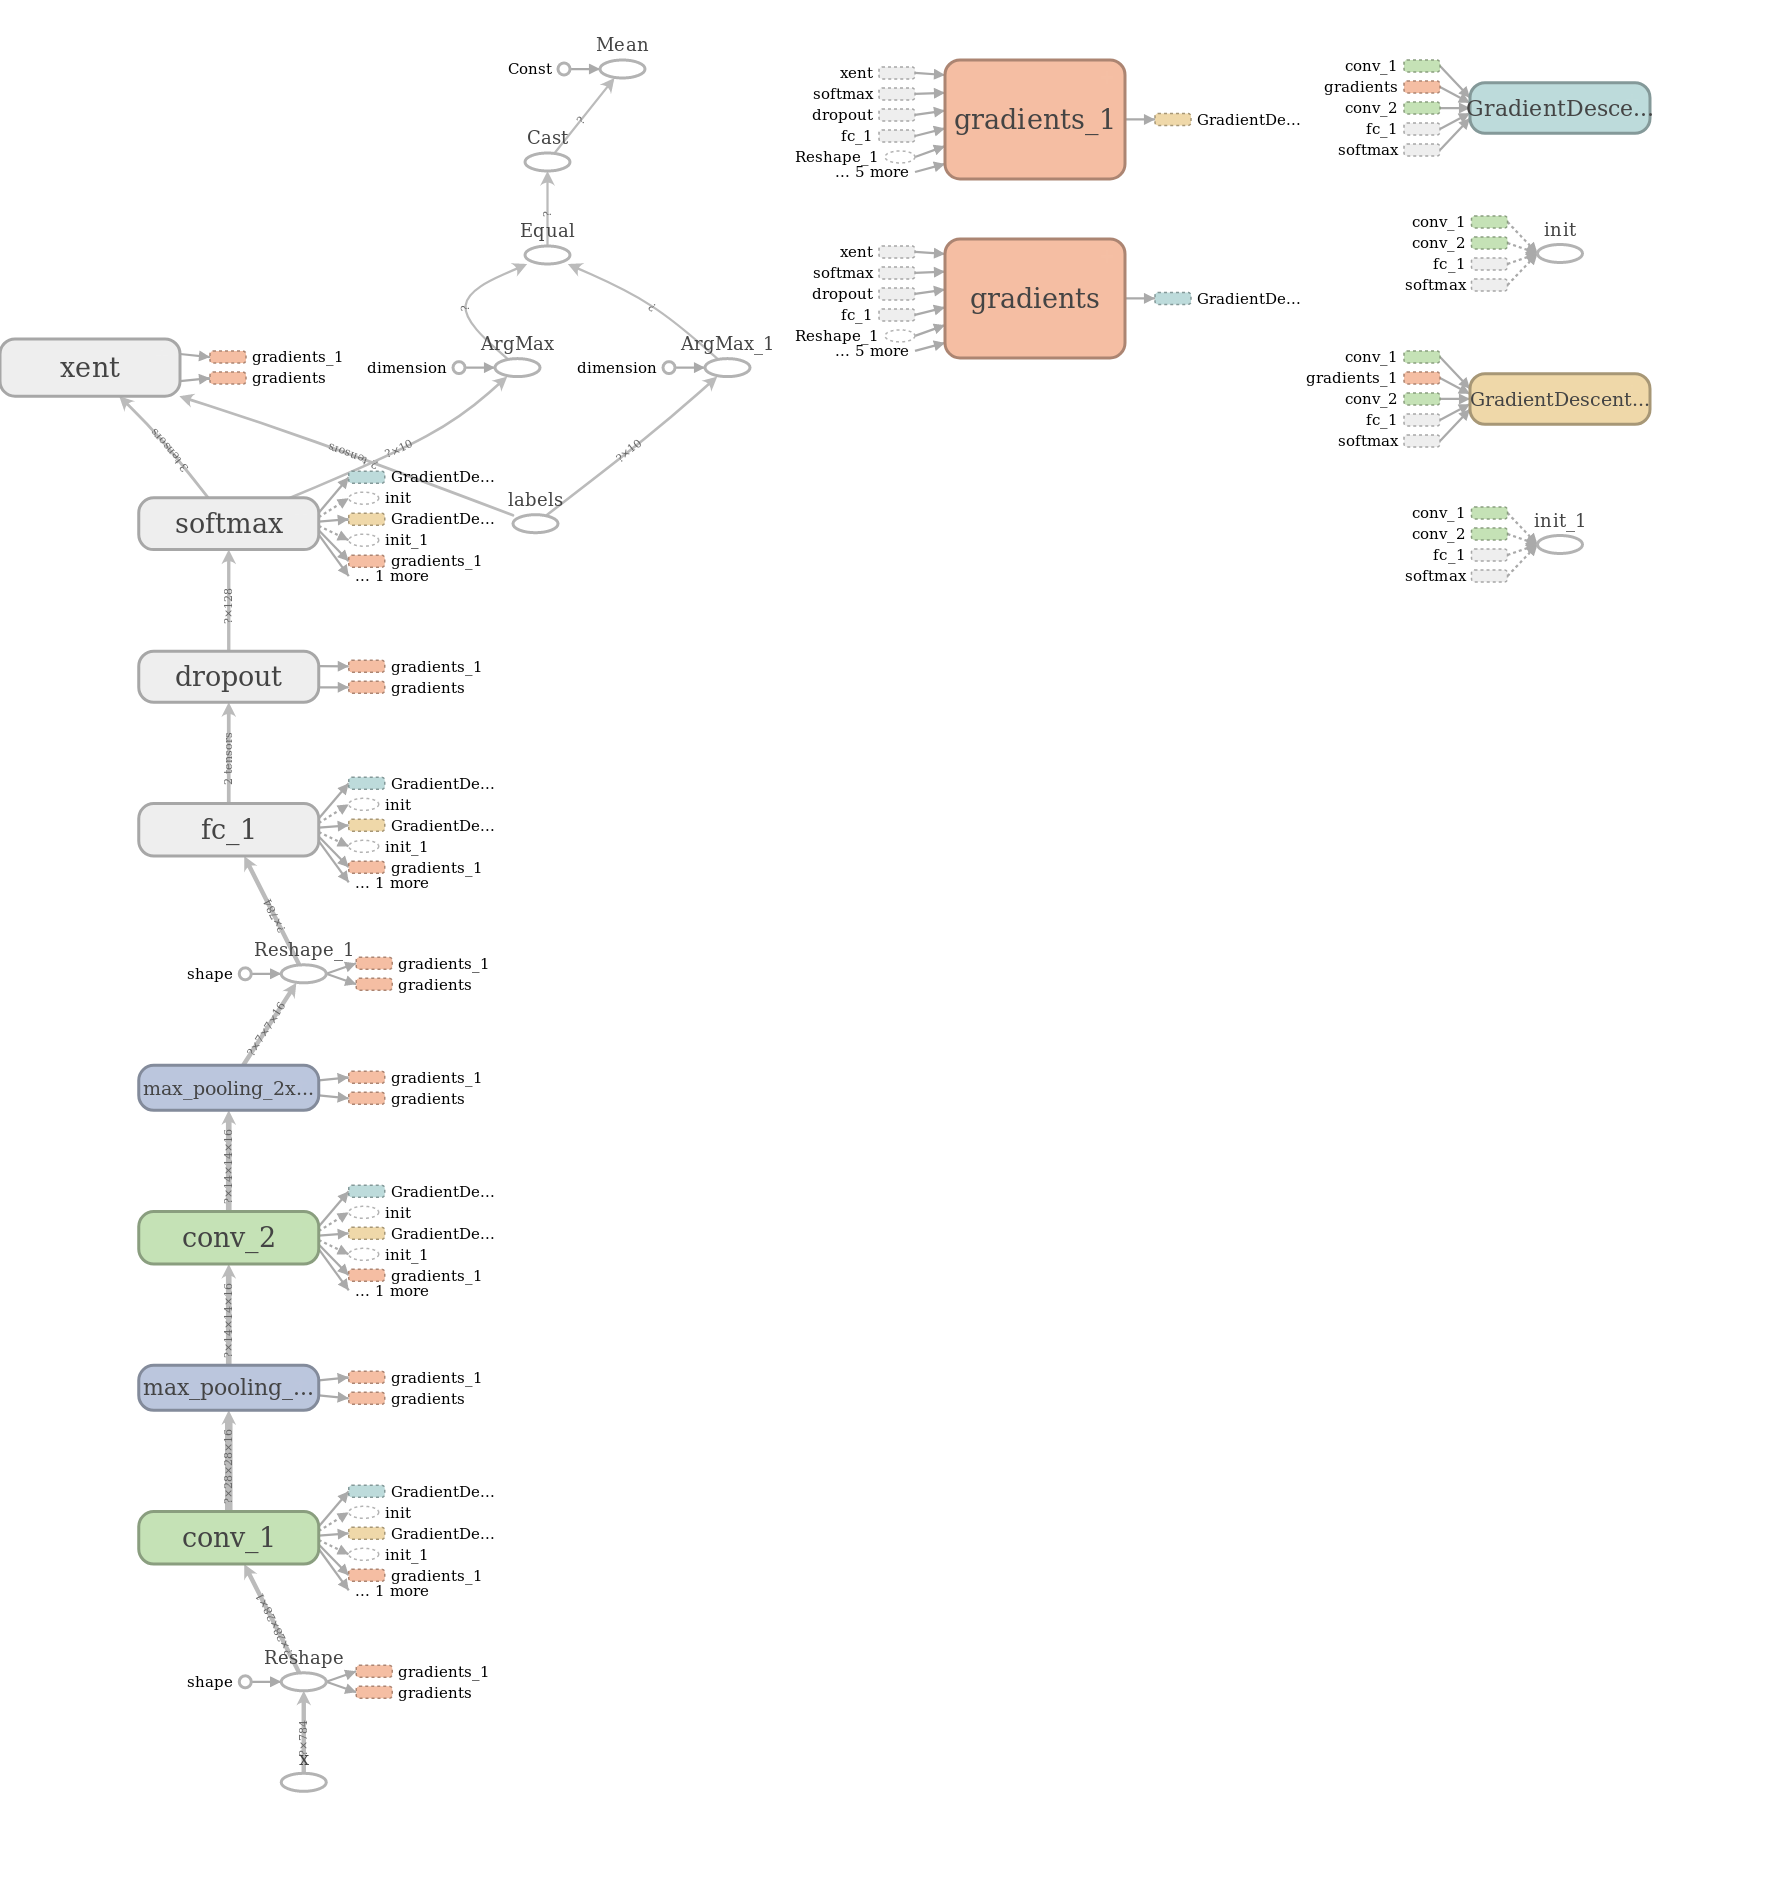
\includegraphics[width=\textwidth,height=9.2cm]{cnn_structure_tb}
	\label{fig:setup}
	\caption{Tensorboard graph of used architecture}
\end{figure}
\vfill


%	
%
%
%
%\subsection{Task 2: Experiments with Learning Rates}
%INSERT PICTURE OF TENSORBOARD GRAPH HERE!
%
%
%
%\subsection{Task3: Runtime comparison CPU vs. GPU with fixed learning rate}
%INSERT PICTURE OF TENSORBOARD GRAPH HERE!
\clearpage
\section{Results}
\subsection{Task 2: Comparison of Learning Rates}

I compared several learning rates with a constant filter size of 16. I added a learning rate of $0.7$ to the learning rates under consideration in order to emphasize the divergent behaviour of the optimiser (SGD) if the learning rate is chosen too high.\\
It can be nicely seen that for very small learning rates, e.g. $0.0001$ the learning does not converge since the steps the optimiser makes during the gradient descent optimisation are too small. Eventually this small learning rate will lead to convergence, but it would take far more epochs (>>20). On the other hand we can see for a rather high learning rate, e.g. $0.7$ the optimisation does not converge, too. On the contrary, it diverges: the steps the optimiser makes are now so big that it comes to an "overshooting" of the minimum. This results in almost constant training/testing accuracy and also the costs will not decrease. Now, convergence is not guaranteed anymore.\\
A rather good result is obtained with the learning $0.1$. It is not to small and not to big and the optimiser manages it find a minimum within the 20 epochs.\\
Overall one can say a CNN can be easy to implement and lead to very good result, but the designer has to have some intuition about good hyperparameters or if he lacks that knowledge, knows how to do a hyperparameter optimisation with for example random search, grid search, hill climbing, etc...

\begin{minipage}[t]{0.33\textwidth}
	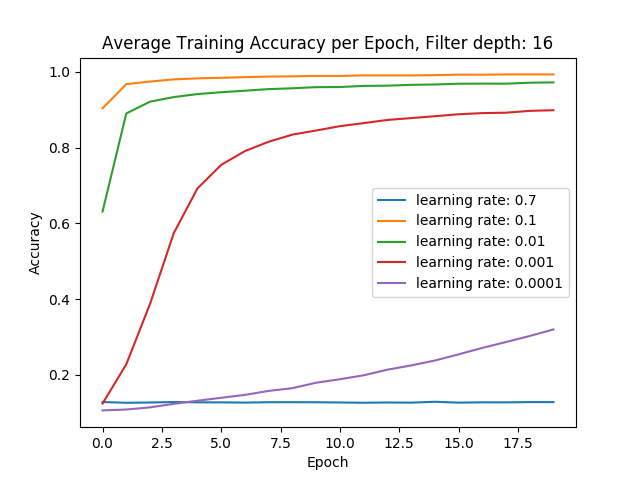
\includegraphics[width=\textwidth,height=6cm]{training_curve}
\end{minipage}
\begin{minipage}[t]{0.33\textwidth}
	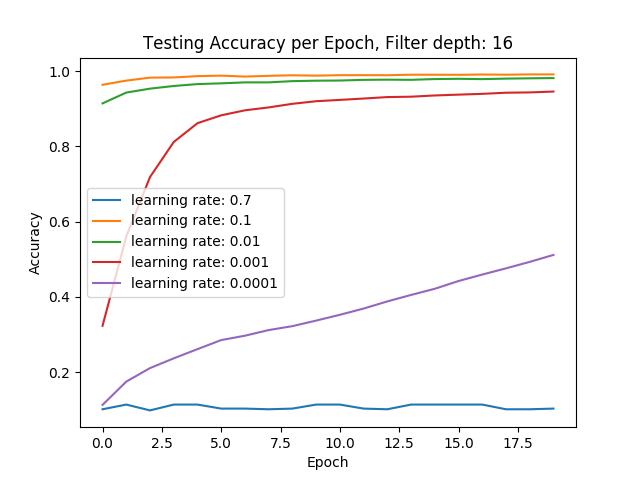
\includegraphics[width=\textwidth,height=6cm]{testing_curve}
\end{minipage}
\begin{minipage}[t]{0.33\textwidth}
	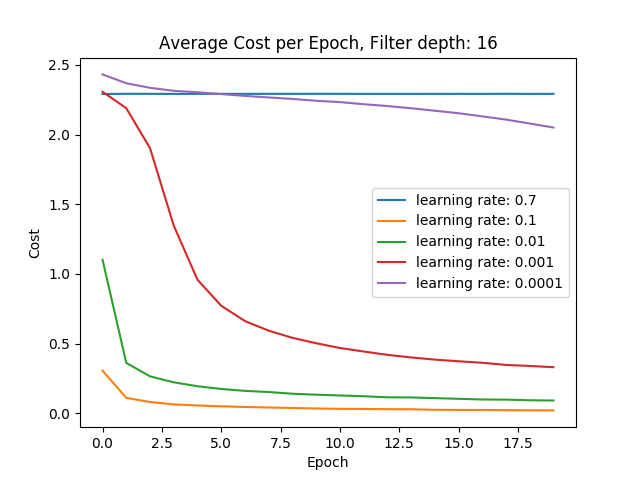
\includegraphics[width=\textwidth, ,height=6cm]{cost_curve}
\end{minipage}
\clearpage
\subsection{Task 3: Runtime Comparison}

The runtime comparison shows that the runtime increases exponentially for the increasing number of filters, since the parameters also increases.
Overall are the GPU runtimes faster than the CPU runtimes.\\


\begin{tabular}{|c|c|c|c|c|}
\hline 
\textbf{CPU} &  &  & &    \\ 
\hline 
\hline
Filter depth & 8 & 16 & 32 & 64   \\ 
\hline 
Parameters & • & • & • & •   \\ 
\hline 
Runtime & 6.3 & 7.8 & 12.7 & 31.   \\ 
\hline
\end{tabular} 
\hfill
\begin{tabular}{|c|c|c|c|c|c|c|}
\hline
\textbf{GPU} &  &  &  &  &  &  \\ 
\hline 
\hline
Filter depth & 8 & 16 & 32 & 64 & 128 & 256 \\ 
\hline 
Parameters & • & • & • & • & • & • \\ 
\hline 
Runtime & • & • & • & • & • & • \\ 
\hline 
\end{tabular} 
\begin{minipage}[t]{0.45\textwidth}
	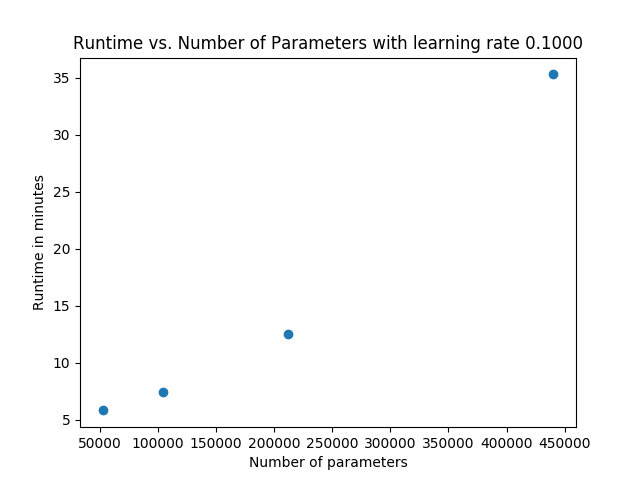
\includegraphics[scale=.5]{runtime_cpu}
	CPU Runtime vs. number of parameters
\end{minipage}
\hfill
\begin{minipage}[t]{0.45\textwidth}
	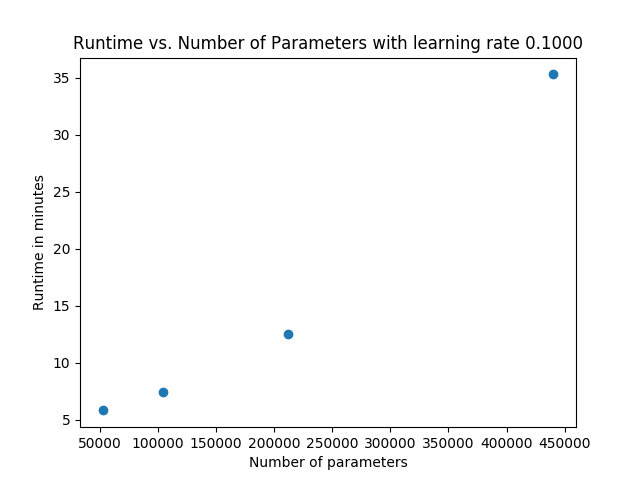
\includegraphics[scale=.5]{runtime_cpu}
	GPU Runtime vs. number of parameters

\end{minipage}




\end{document}